\section{Approach Adopted}

edw

to keimeno

pou tha leei

panw katw

ti ginetai

s'auto to kefalaio

DHLADH THA ESTIAZEI STO WS 'H LDAP

\newpage

\subsection{implementation of performance analysis of
distributes systems in GMA}
na perigrapsw to paper: \cite{balatonuse}
requirements

very large volume of data

measurement data must be accurate and consistent

problems

time synchronisation

time measurments must be accurate

time measurements must be consistent.

implementation

consumer registers interest

trace events generation

producers query IS for consumer

producers subscribe to consumers

consumer get events

\newpage

\section{Design Methods}
\subsection{Recommendations and standards}
\subsubsection{Grid Monitoring Architecture}
\nomenclature{GMA}{Grid Monitoring Architecture}
%% TODO producer-consumer plot
\newpage

\subsubsection{R-GMA}
%% TODO R-GMA literature
\newpage

\nomenclature{R-GMA}{Relational Grid Monitoring Architecture}
\subsubsection{XML schema}
\subsubsection{GLUE}
gained wide acceptance given its adoption by Globus MDS3
\nomenclature{GLUE}{Grid Laboratory Uniform Environment}
\newpage

\begin{figure}[htb]
\centering
 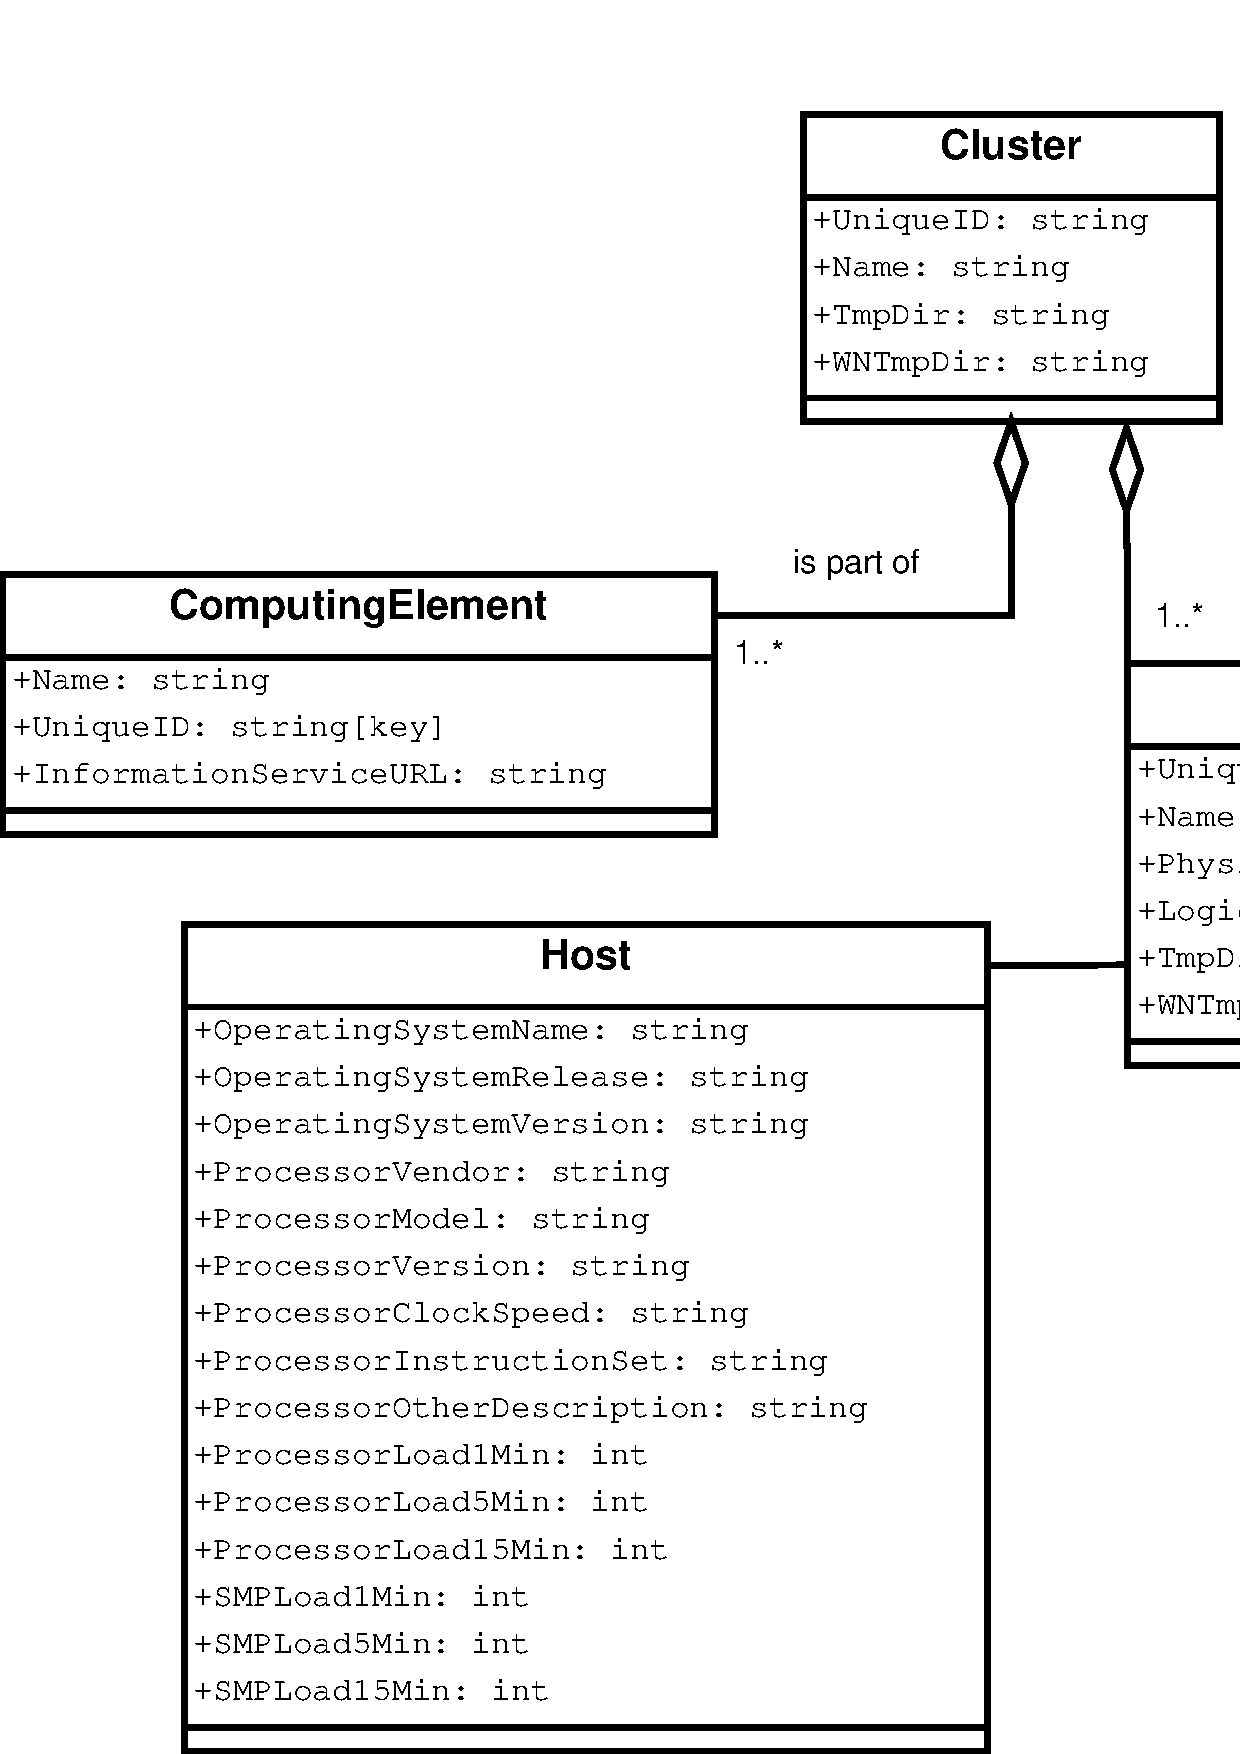
\includegraphics[width=5in]{images/gluece_ext.pdf}
\caption{GLUE schema 2.0 extention for Host and SMP Load}
\label{figure:gluece_ext}
\end{figure}

\newpage

\subsection{Information Infrastructure}
% TODO to MDS me dika mou logia
``Performance''.  The applications of interest to us frequently 
operate on  a  large scale  (e.g.,  hundreds  of  proces- 
sors) and have demanding performance requirements. 
Hence, an information infrastructure must permit rapid 
access to frequently used configuration information. It 
is not acceptable to contact  a  server  for every  item: 
caching is required.
``Scalability and cost''. The infrastructure must scale to large
numbers of components and permit concurrent access
by many entities. At the same time, its organization
must permit easy discovery of information. The human
and resource costs (CPU cycles, disk space, network
bandwidth) of creating and maintaining information
must also be low, both at individual sites and in total.
``Uniformity''. Our goal is to simplify the development of
tools and applications that use data to guide configuration
decisions. We require a uniform data model
as well as an application programming interface (MI)
for common operations on the data represented via that
model. One aspect of this uniformity is a standard representation
for data about common resources, such as
processors and networks.
``The X.500 standard'' defines a directory service
that can be used to provide extensible distributed directory
services within a wide area environment. A directory service
is a service that provides read-optimized access to general
data about entities, such as people, corporations, and computers.
X.500 provides a framework that could, in principle,
be used to organize the information that is of interest to us.
\cite{mds1}
\newpage

\section{Data-acquisition Systems}
plugins that take metrics (SAM) and send results to nagios:

https://tomtools.cern.ch/confluence/display/SAMDOC/Grid+probes

http://nationalgridservice.blogspot.com/2010/10/nagios-myegee-and-myegi.html

4 layers to performance investigation:
\begin{enumerate}
  \item Storage elements
  \item Sites
  \item VOs
  \item Middleware
\end{enumerate}
3 benchmarking categories
\begin{enumerate}
  \item micro-benchmarks
  \item micro-kernels
  \item application kernels
\end{enumerate}
Benchmarking

HPL
\cite{gridbench}

CE performance
free processors
MFLOPS
MIPS (instructions per second)
free RAM

SE performance
IOPS
free space

EGI accounting portal: CPU usage metrics aggregated for accounting.
\newpage

\subsection{Metrics}

{\bf CPU load} is taken using the pseudo /proc/loadavg file which in turn is
filled by Linux kernel's CALC\_LOAD macro. This function takes 3 parameters.
The load-average bucket, a $y$ constant that is calculated using formula
\[
y=\frac{2^{11}}{2^{((5log_2(e))/60x)}}
\]
for values $x=1$, $x=5$ and $x=15$ (where x represent the minutes and y the
exponent constant), and the number of how many processes are in the queue, in
running or uninterruptible state.

\begin{figure}[htb]
\centering
 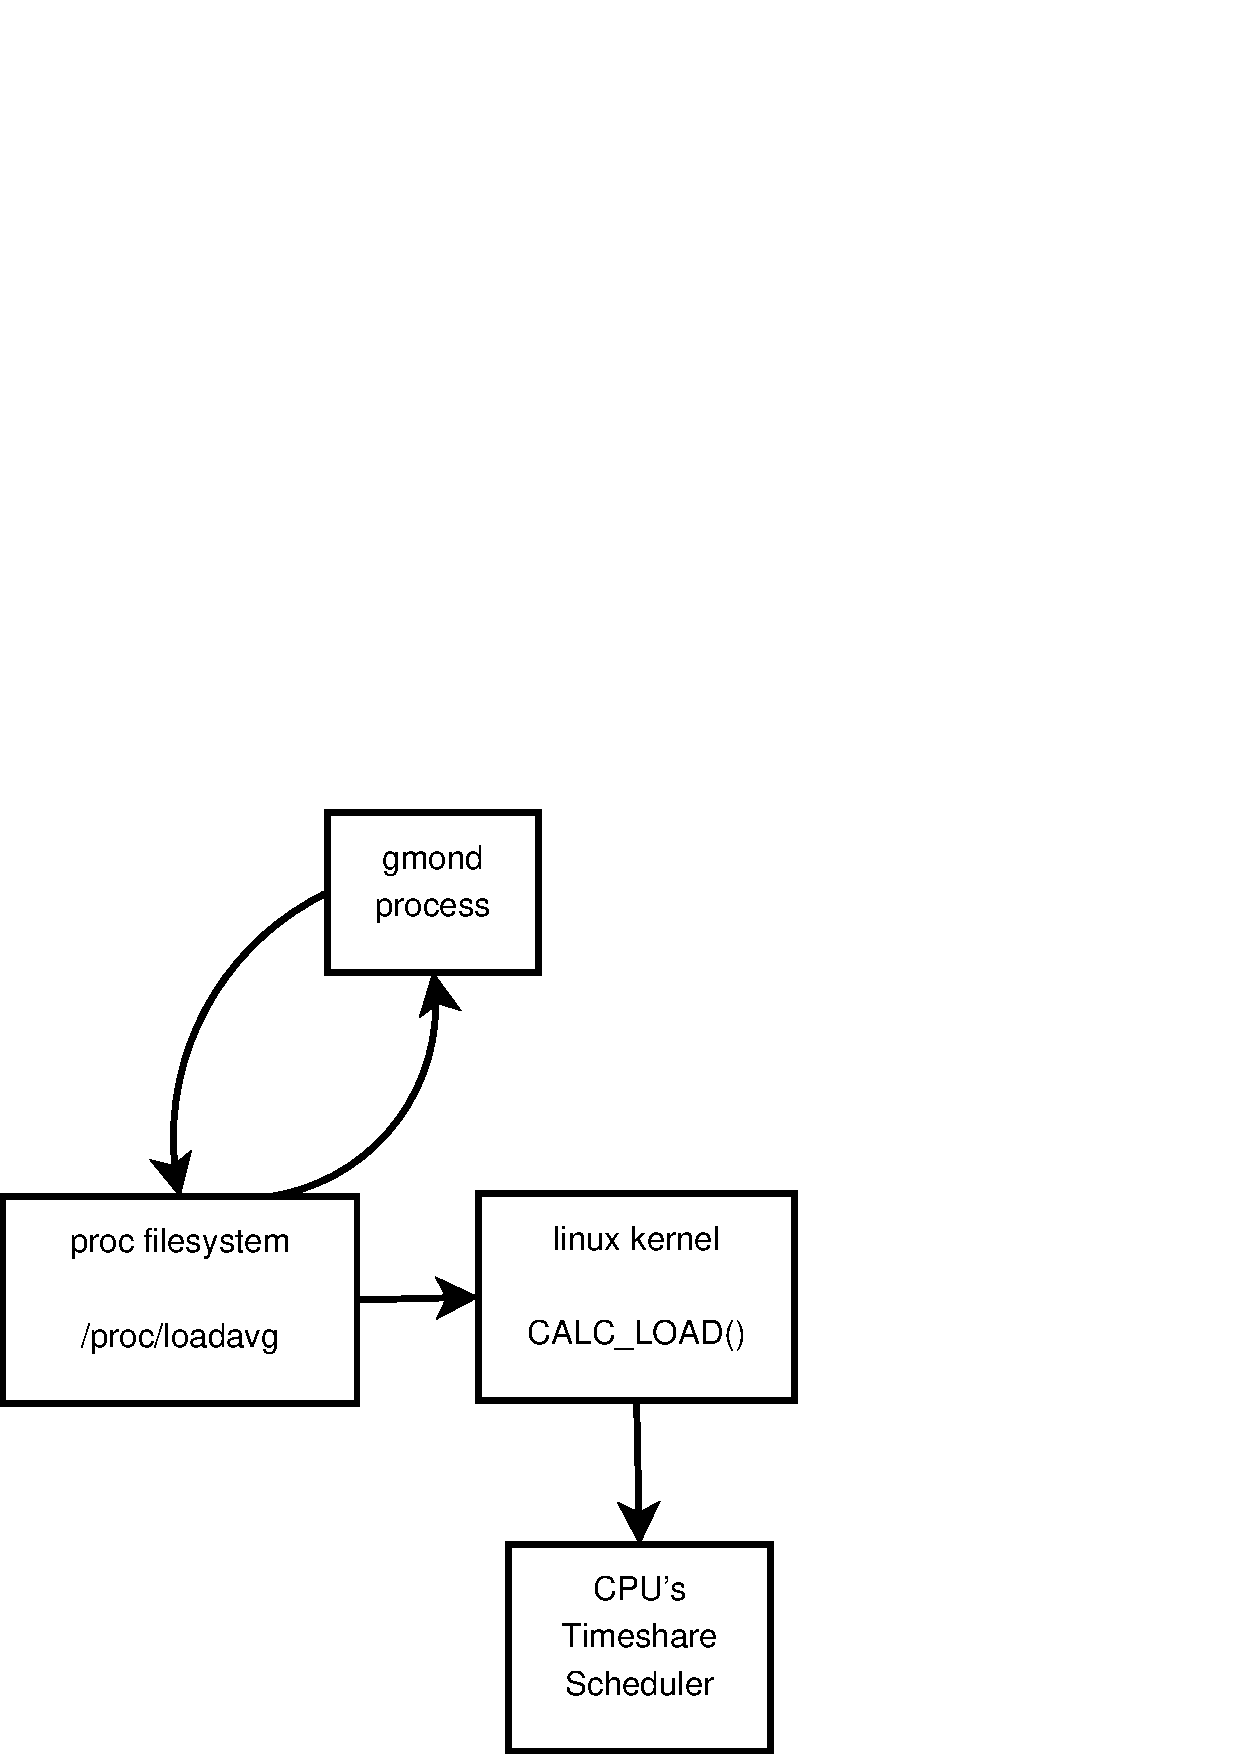
\includegraphics[width=3in]{images/calc_load.pdf}
\caption{Load Average calculation}
\label{figure:calc_load}
\end{figure}

\newpage

\subsection{Ganglia}
enw to ganglia to kanei etsi
\newpage

\begin{figure}[htb]
\centering
 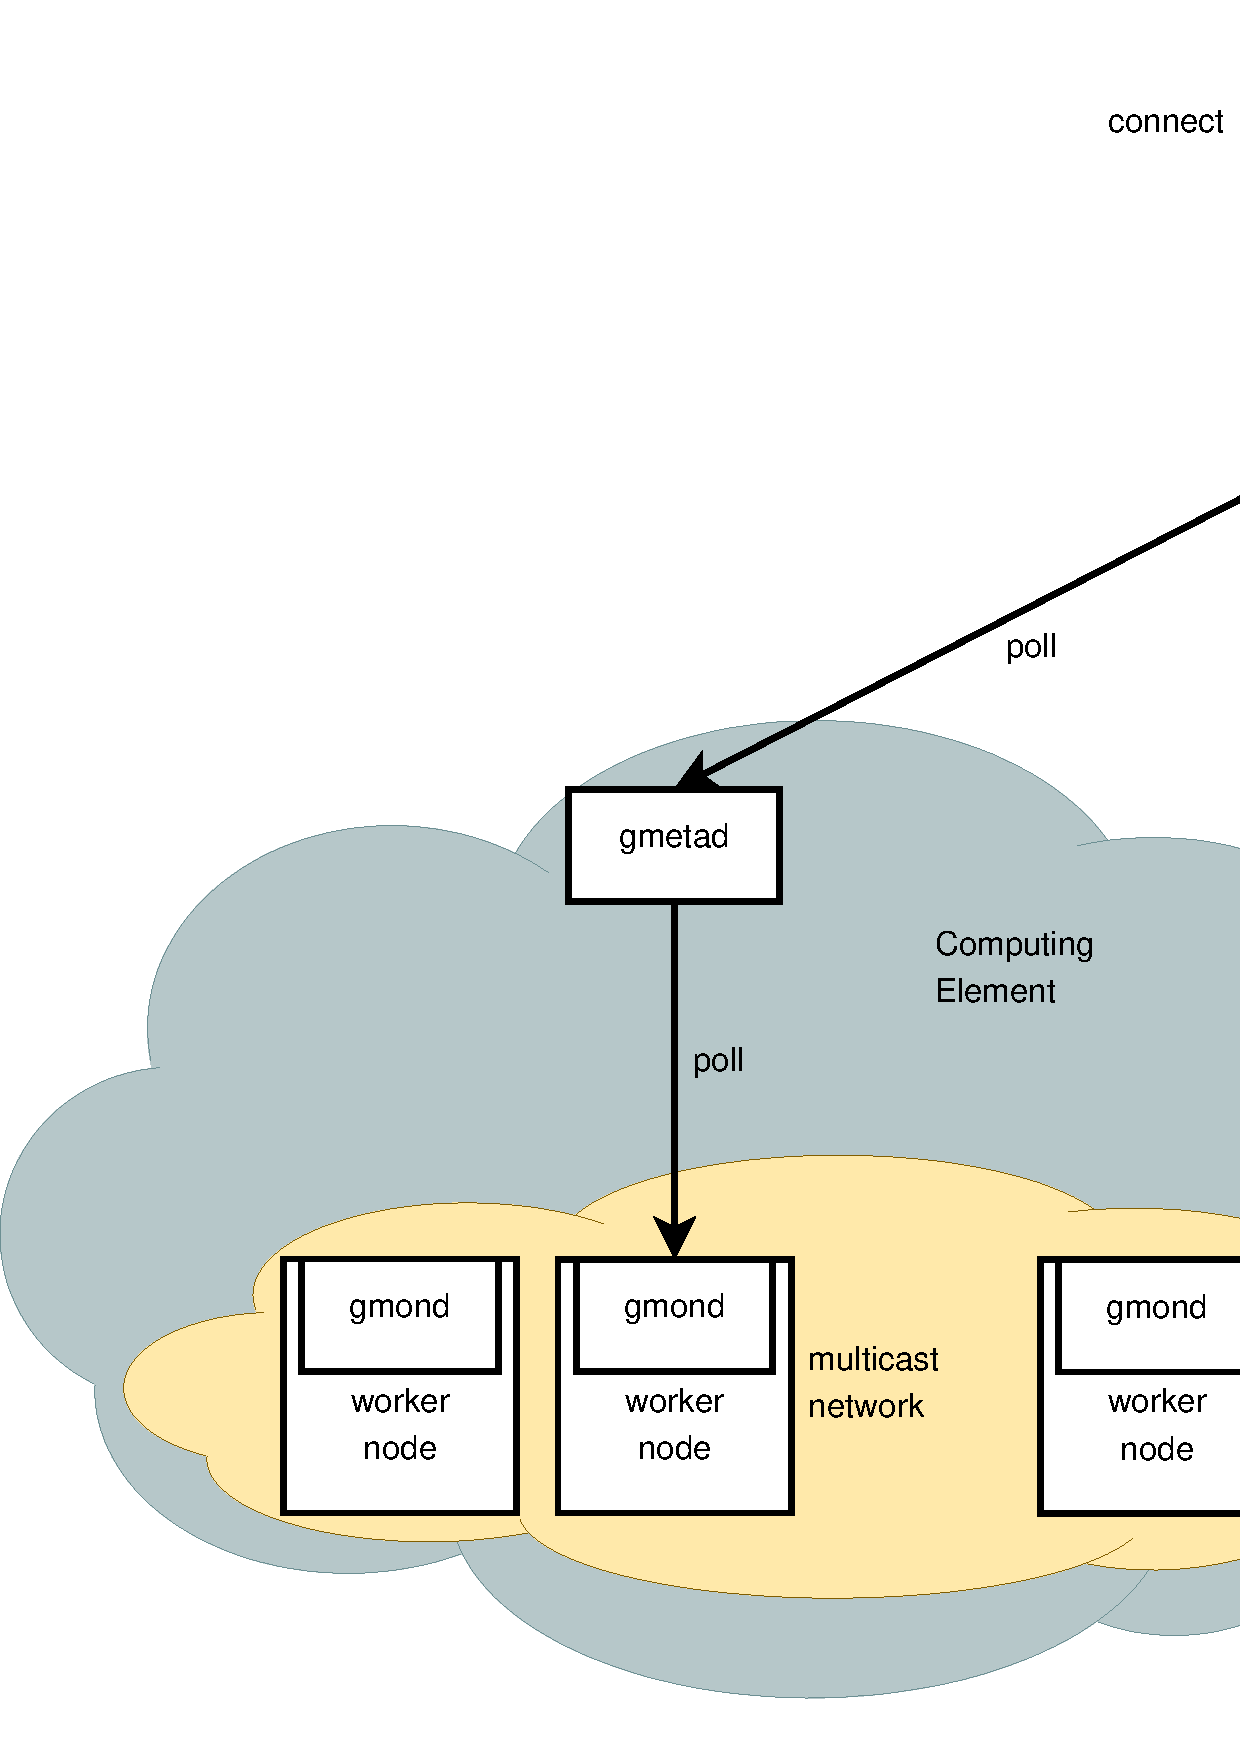
\includegraphics[width=6in]{images/ganglia_data_flow.pdf}
\caption{Ganglia Data Flow}
\label{figure:ganglia_dataflow}
\end{figure}
\newpage

\subsection{Nagios}
msg-to-handler msg-nagios-bridge
\newpage

nagios2metric
\newpage

\subsection{Ganglia to Nagios}
check\_ganglia
\begin{figure}[htb]
\centering
 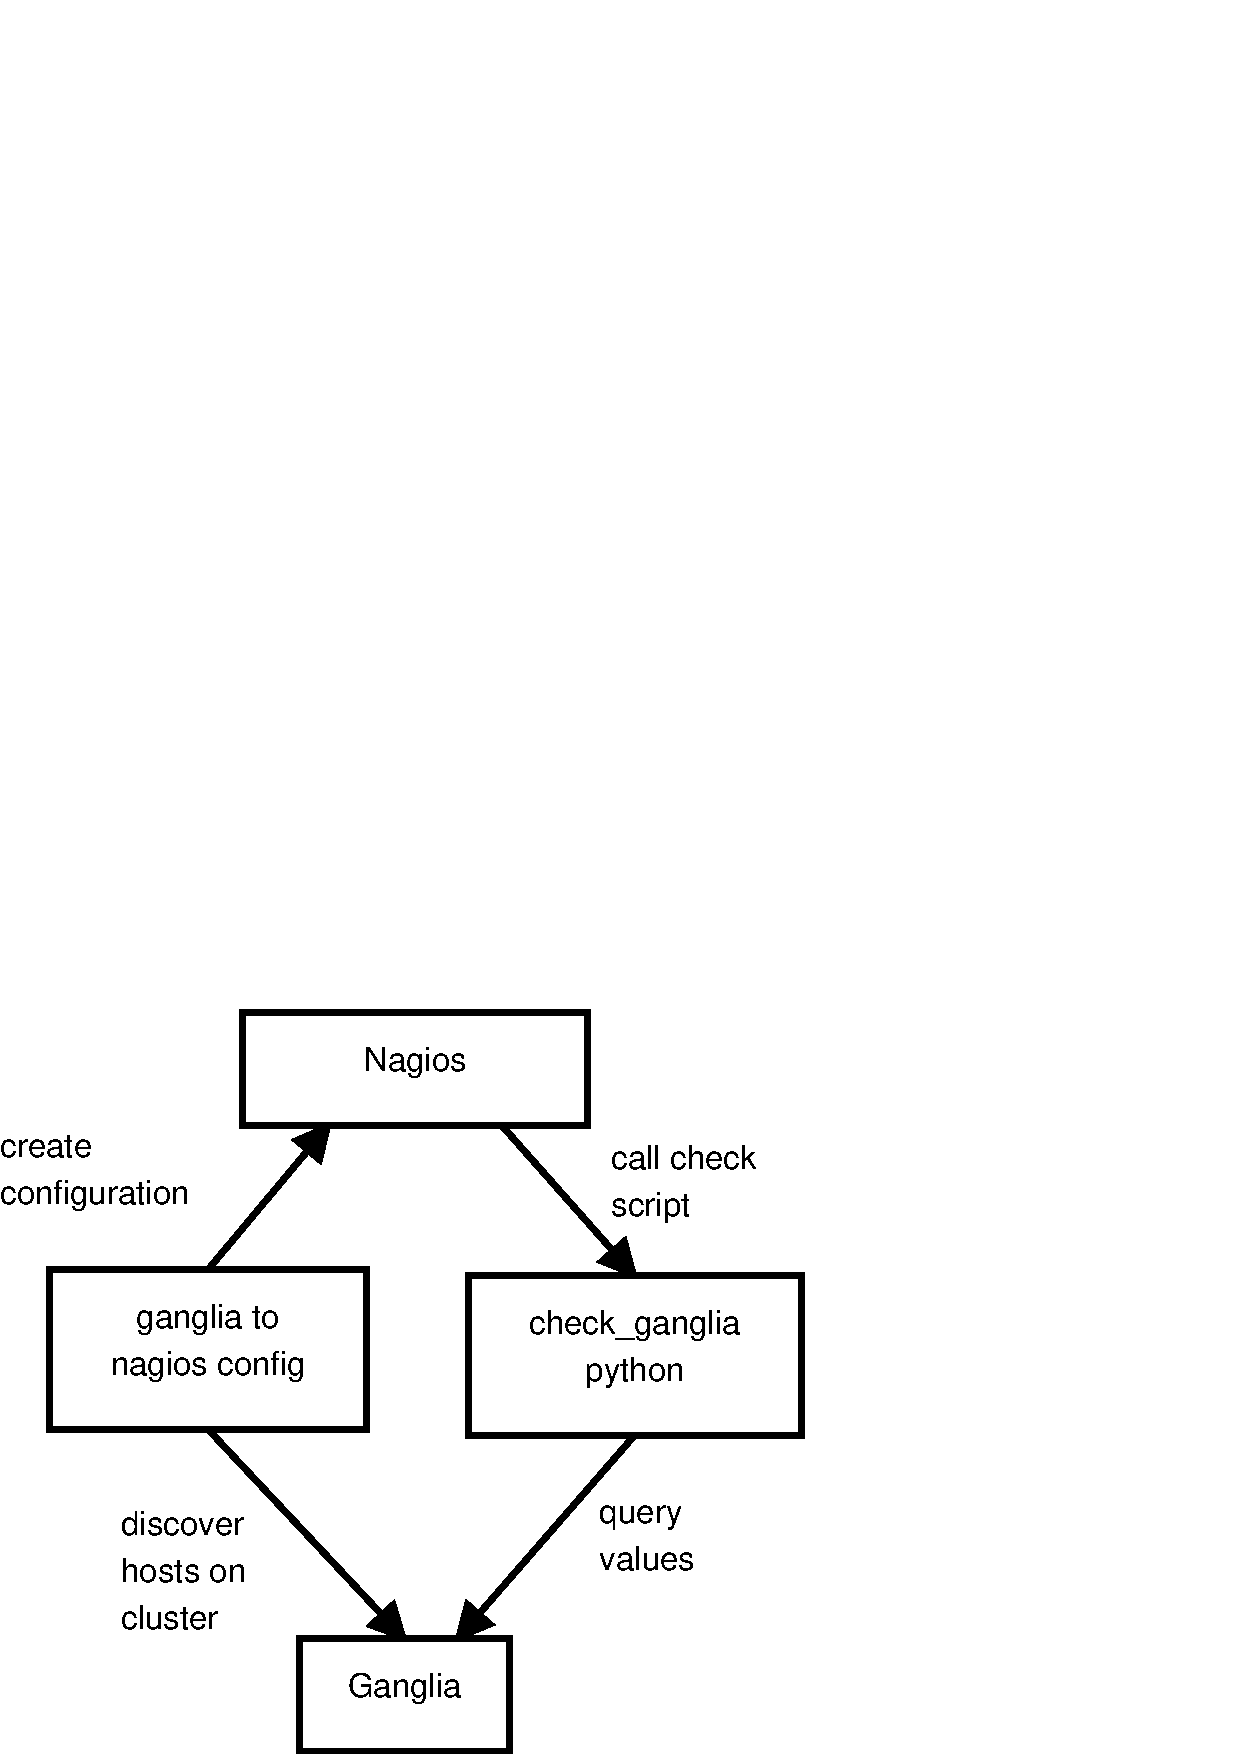
\includegraphics[width=2in]{images/nagios_check_ganglia.pdf}
\caption{Nagios configuration and check ganglia values}
\label{figure:nagios_ganglia}
\end{figure}
\newpage

\subsection{pnp4nagios}

Bulk Mode with NPCD
NPCD:
spool directory to process bulk data
create graphs using RRDTOOL

\begin{figure}[htb]
\centering
 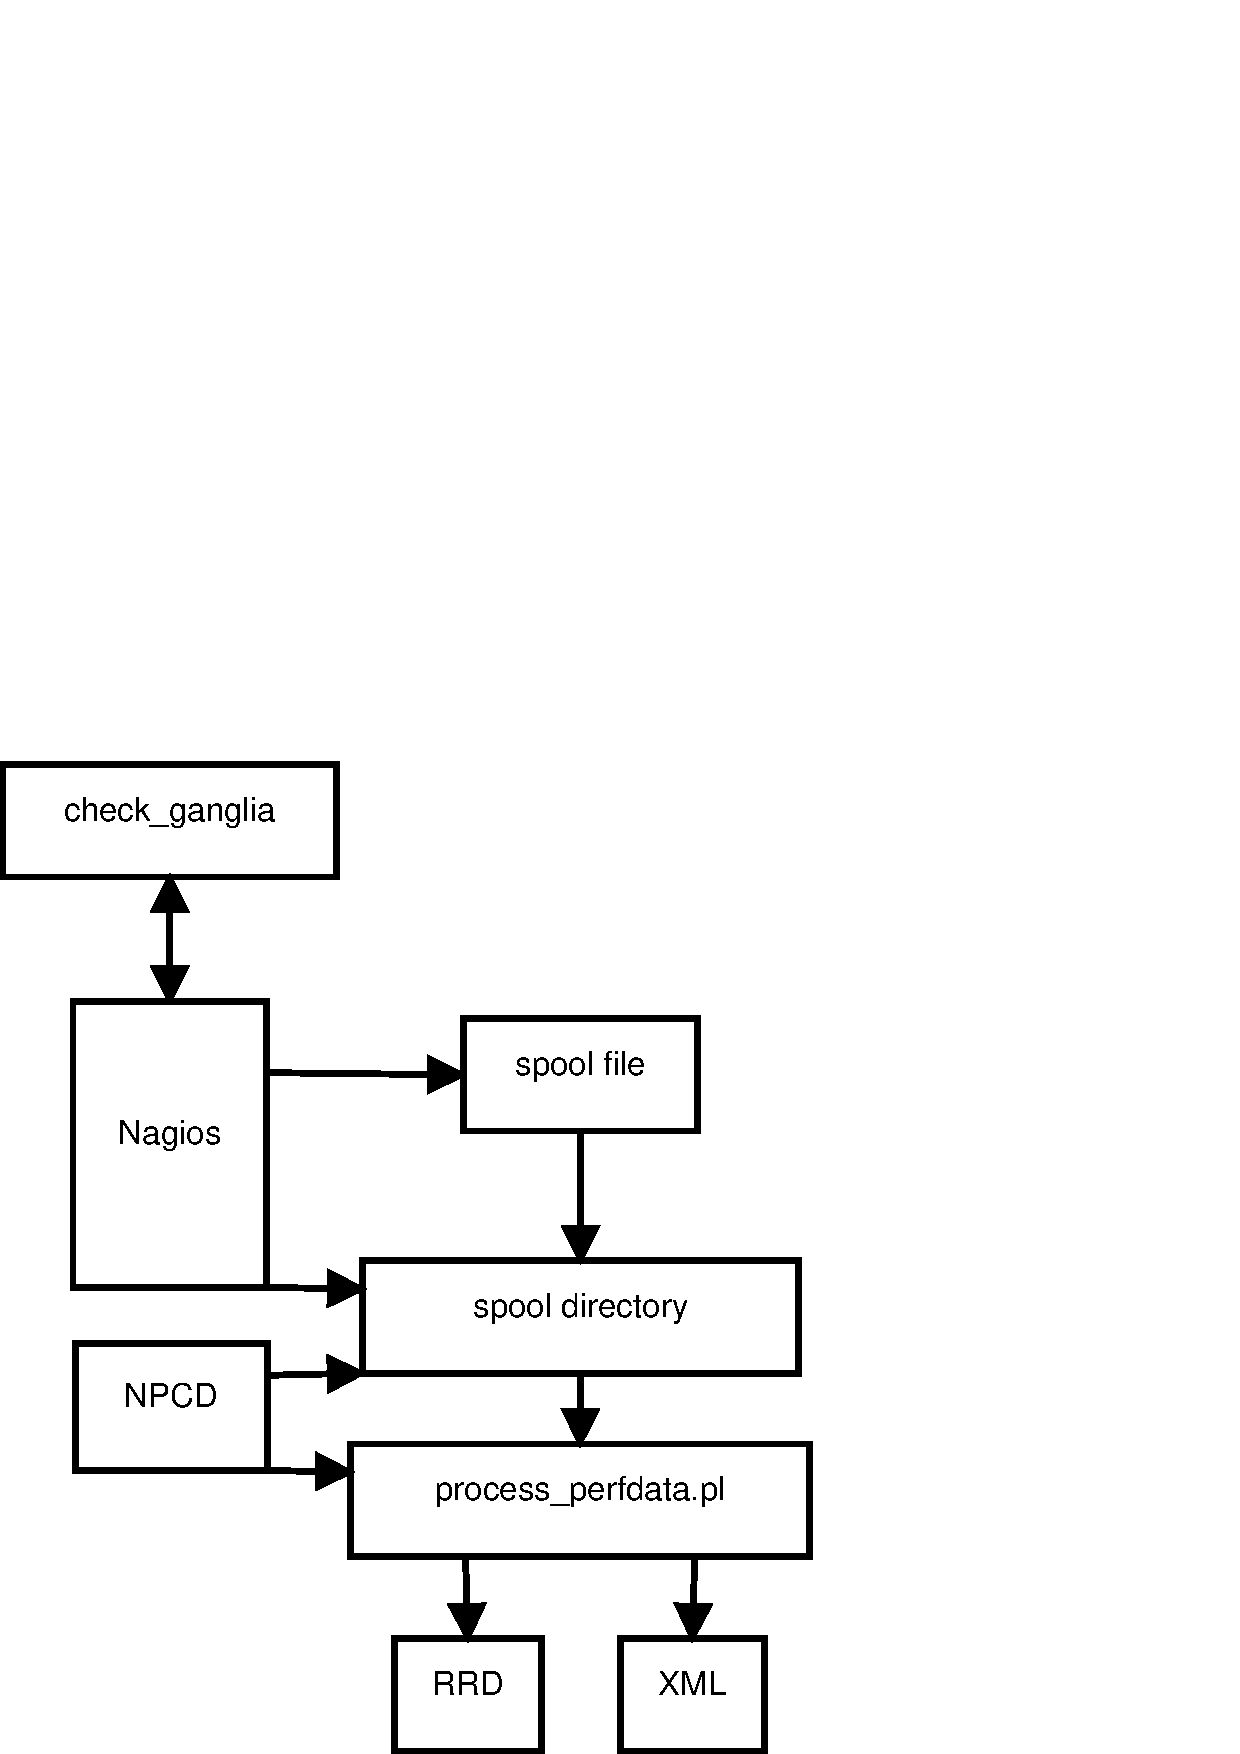
\includegraphics[width=3in]{images/npcd_pnp4nagios.pdf}
\caption{PNP 4 Nagios data flow}
\label{figure:pnp4nagios}
\end{figure}
\newpage

\section{Range of cases examined - Metrics}
% here there will be an enumeration of metrics, gmond, etc

Grid performance can be measured using benchmark tools in different levels of
the grid architecture, using the micro-benchmarks at the Worker Node level, the
Site (CE) level and the Grid VO level. Various benchmarks exist in these
levels, using different libraries and algorithms, such as  This project focuses
on mathematically compute of the performance of a grid based on the metrics that
are taken at the Worker Node level.

Different metrics and benchmarks exist, such as the measurement of
the performance of CPUs in {\bf MIPS using EPWhetstone} and the evaluation of
the performance of a CPU in {\bf FLOP/s and MB/s using BlasBench}. GridBench
\cite{gridbench} provides a framework to collect those metrics using its own
description language, {\bf GBDL}.

GcpSensor \cite{gcpsensor} introduce a new performance metric called WMFLOPS. It
uses PAPI \cite{papi} (Performance API) to access the hardware performance
counters. For data distribution it uses MDS information system which provides
dynamic metrics for CPU load average, one for 1, for 5 and for 15 minutes load.
\newpage

% TODO ganglia to MDS
\section{Publish to Information System}

\subsection{LDAP based - MDS/BDII}
\begin{enumerate}
  \item Python ganglia client script:
  http://globus.org/toolkit/docs/2.4/mds/gangliaprovider.html
  \item Perl gaglia-IP tool:
  
  http://www.star.bnl.gov/public/comp/Grid/Monitoring/SimpleGangliaIP.html
  
  http://www.star.bnl.gov/public/comp/Grid/Monitoring/ganglia\_ip

\end{enumerate}

\newpage
Glue schema

GlueCluster
GlueClusterTop
GlueGeneralTop
GlueHost
GlueHostArchitecture
GlueHostMainMemory
GlueHostNetworkAdapter
GlueHostOperatingSystem
GlueHostProcessor
GlueHostProcessorLoad
GlueHostSMPLoad
GlueSubCluster
GlueTop

Perl:
\begin{lstlisting}
$[root@mon ~]# ./ganglia_ip -h mon -p 8649 -o mds
\end{lstlisting}

Python:
\begin{lstlisting}
$[root@mon ~]# /opt/ganglia/bin/ganglia --format=MDS
\end{lstlisting}

\newpage

\subsection{Web Service based - WSRF}
\subsubsection{container}
using WSRF (GT4, information services, information providers)
Ganglia Resource Provider
MDS Index Service
GLUE CE 

OASIS standard

container
\newpage
\subsection{information provider}
wssd

kai

rp xml

\newpage
\subsubsection{XPath}
example queries
\subsubsection{XSLT}
my note: WSRF is GLUE 2.0 schema CE compatible
\begin{verbatim}
/opt/globus/etc/globus_wsrf_mds_usefulrp/ganglia_to_glue.xslt

<glue:ProcessorLoad>

<xsl:attribute name="glue:Last1Min">
  <xsl:call-template name="emitProperNumeric">
    <xsl:with-param name="numeric" 
    select="floor(100 * METRIC[@NAME='load_one']/@VAL)"/>
  </xsl:call-template>
</xsl:attribute>

<xsl:attribute name="glue:Last5Min">
  <xsl:call-template name="emitProperNumeric">
    <xsl:with-param name="numeric" 
    select="floor(100 * METRIC[@NAME='load_five']/@VAL)"/>
  </xsl:call-template>
</xsl:attribute>

<xsl:attribute name="glue:Last15Min">
  <xsl:call-template name="emitProperNumeric">
    <xsl:with-param name="numeric" 
    select="floor(100 * METRIC[@NAME='load_fifteen']/@VAL)"/>
  </xsl:call-template>
</xsl:attribute>

</glue:ProcessorLoad>
\end{verbatim}
\newpage

\subsubsection{WebMDS}
webmds